%  PHDTHESIS TEMPLATE FILE
%  Adopted from Thomas Fabricius and Henrik Aalborg Nielsen
%  Jan Larsen, IMM, DTU, Nov 2003 ver 1.0
%  Updated by Finn Kuno Christensen, fkc@imm.dtu.dk Aug 15, 2008

%  COMPILATION STEPS USING INVOLVING A PS FILE
\documentclass[10pt,twoside,dvips]{book}
%  latex phdthesis.tex
%  dvips -D600 -Pamz -Pcmz -j0 phdthesis.dvi -o phdthesis.ps
%  ps2pdf -sPAPERSIZE=b5 phdthesis.ps phdthesis.pdf (or use Acrobat Distiller)

%  COMPILATION STEP USING PDFLATEX
%\documentclass[10pt,twoside]{book}
%  pdflatex phdthesis.tex

%%%%%%%%%%% MODIFY THESE LINES ONLY %%%%%%%%%%%%%%%%%%%%%%%%%%%%%%%%%%%%%%%%%%%%%%%%%%%%%%%%%
\usepackage[latin1]{inputenc}

\def\thesisyear{2010} % Year thesis submitted
\def\thesisnumber{1}  % Only number no year
\def\thesisauthor{Kasper Bj�rn Nielsen} % Thesis author
\def\thesistitle{Failsafe Control for DTUSat2} % Title of thesis
\def\thesiskeywords{Software technology}
\def\thesisversion{print} %OBSOBS choose this for printed version send to printing
%\def\thesisversion{net} %OBSOBS choose this for the net version for the web and publication database
%%%%%%%%%%%%%%%%%%%%%%%%%%%%%%%%%%%%%%%%%%%%%%%%%%%%%%%%%%%%%%%%%%%%%%%%%%%%%%%%%%%%%%%%%%%%%

%%%%%%%%%%%%%%% DO NOT MODIFY START %%%%%%%%%%%%%%%%%%%%%%%%%%%%%%%%%%%%%%%%%%
\def\thesisISSN{0909-3192}
\def\ttitle{{\sf\textbf{\thesistitle}}}
\def\thesisdef{IMM-PHD-\thesisyear-\thesisnumber}
\usepackage{hyperref}
\def\printversion{print}
\ifx\thesisversion\printversion
  \special{papersize=176mm,250mm}
  \hypersetup{pdftitle={\thesistitle},
              pdfauthor={\thesisauthor},
              pdfsubject={\thesisdef},
              pdfkeywords={\thesiskeywords},
              breaklinks,
              bookmarksopen,
              bookmarksnumbered}
\else
  \hypersetup{pdftitle={\thesistitle},
              pdfauthor={\thesisauthor},
              pdfsubject={\thesisdef},
              pdfkeywords={\thesiskeywords},
              colorlinks,
              linkcolor=blue,
              breaklinks,
              bookmarksopen,
              bookmarksnumbered}
\fi


%%%%%%%%%%%%%% DO NOT MODIFY BELLOW START%%%%%%%%%%%%
\usepackage[latin1]{inputenc}
\usepackage[english]{babel}
\usepackage{fancyheadings}
\usepackage{amsmath,amssymb,latexsym,epic,eepic,epsfig,graphics,psfrag}
\usepackage{theorem}
\usepackage{immthesislayout}

\newcommand{\papertitle}{}
\setcounter{tocdepth}{1} % 1 in final version 10 for debugging
\setcounter{secnumdepth}{3} % subsubsections get a number when this is 3

% PDF:
%\usepackage[pdftitle={PARAMETRIC AND NON-PARAMETRIC SYSTEM MODELLING},
%            pdfauthor={Henrik Aalborg Nielsen, IMM, DTU},
%            breaklinks,
%            bookmarksopen,
%            bookmarksnumbered]{hyperref}
%\hypersetup{pdftitle={\ttitle},
%%            pdfsubject={\thesisdef},
%            pdfkeywords={\thesiskeywords},
%            breaklinks,
%            bookmarksopen,
%            bookmarksnumbered}

\begin{document}
\thispagestyle{empty}
\vspace*{\fill}
\begin{center}
{\huge\ttitle}\\*[2.5cm]
\Large\sf\thesisauthor\\*[4.5cm]
\small\sf Kongens Lyngby \thesisyear\\
\small\sf IMM-PHD-\thesisyear-\thesisnumber
\end{center}
\vspace*{\fill}
\newpage
\thispagestyle{empty}
\vspace*{11cm}
{\sf Technical University of Denmark}\\
{\sf Informatics and Mathematical Modelling}\\
{\sf Building 321, DK-2800 Kongens Lyngby, Denmark}\\
{\sf Phone +45 45253351, Fax +45 45882673}\\
{\sf reception@imm.dtu.dk}\\
{\sf www.imm.dtu.dk}

\vspace*{2.5cm}
\def\empty{}
\ifx\thesisISBN\empty
  {\sf IMM-PHD: ISSN \thesisISSN}
\else
  {\sf IMM-PHD: ISSN \thesisISSN, ISBN \thesisISBN}
\fi


\frontmatter
\pagenumbering{roman}

%%%%%%%%%%%%%%% DO NOT MODIFY END %%%%%%%%%%%%%%%%%%%%%%%%%%%%%%%%%%%%%%%%%%%%

%%%%%%%PREFACE CHAPTERS INCLUDE%%%%%%%%%%%%%%%%%%%%%%%%%%%%%%%%%%%%%%%%%%%%%%

\chapter{Abstract}

The DTUSat-2 project is a student satellite project at DTU. Any software being run on the satellite could potentially make the satellite unresponsive if a serious error occured. Therefore, a failsafe mode has been developed which should catch theses failures so that the DTUSat-2 staff can investigate errors and prevent them from happening again by uploading new software.
To operate the failsafe mode the staff needs both a console tool and a graphical user interface. It is the purpose of this project to investigate possible solutions and produce the software necesarry for the staff to be able to operate the satellite when in failsafe mode.

\markboth{}{}
\chapter{Preface}

This Bachelor thesis was accomplished at the Department of Informatics and Mathematical Modelling (IMM), at the Technical University of Denmark (DTU), during the period 1st of February 2010 to the 30th of June 2010. The project was supervised by Associate Professor Hans Henrik L�vengreen of the IMM department at DTU.

This thesis documents the Failsafe Control for DTUSat-2 software. It is aimed at the DTUSat-2 staff and should give any staff member a thorough overview of the requirements, design decisions, implementation specifics, test results, installation instructions and operating instructions of the software produced.

I would like to thank Hans Henrik L�vengreen for his advice, guidance and enthusiasm throughout the project. Also a big thanks to my friends and my family for their support and advice.
\\ \\
Lyngby, June 2010
\\ \\
Kasper Bj�rn Nielsen, s052808

\markboth{}{}

%%%%%%%PREFACE CHAPTERS INCLUDE%%%%%%%%%%%%%%%%%%%%%%%%%%%%%%%%%%%%%%%%%%%%%%

\newpage\mbox{}\newpage
\chaptermark{Contents}
\renewcommand{\sectionmark}[1]{\markright{#1}}
\sectionmark{Contents}
\addtolength{\parskip}{-\baselineskip}
\tableofcontents
\addtolength{\parskip}{\baselineskip}
\renewcommand{\sectionmark}[1]{\markright{\thesection\ #1}}

\mainmatter
% Chapter 1, 2, ...
%%%%%%%MAIN CHAPTERS INCLUDE%%%%%%%%%%%%%%%%%%%%%%%%%%%%%%%%%%%%%%%%%%%%%%

%\chapter{Introduction}

The DTUSat-2 is a student satellite project of several departments at DTU. The goal of the project is to implement a spaceborne radio-tracking system capable of locating birds on intercontinental migration routes.
When the satellite has been launched and is orbiting earth, it is practically impossible to press a reset button in case of a hardware or software failure. Therefore, unforseen failures that make the satellite unresponsive, must be handled. This is achieved by constantly monitoring for failures and unresponsiveness.
\\ \\
There are two main programs on the satellite. The nominal mode, which is the full functioning autonomous program that normally runs on the satellite. This mode performs the tasks necessary for tracking birds.
\\ \\
If a failure is detected the software will reboot into the unautonomous failsafe mode which is a small program consisting of just 20 commands. In this mode it is possible to investigate what went wrong and to upload new software.
\\ \\
Operating software to the satellite's nominal mode have already been developed. There is a console program called fsterm which was used in DTUSat-1 project to operate the failsafe mode, but this program is no longer sufficient as new commands have been added and a graphical user interface (GUI) has become a requirement.

\section{Thesis Statement}
The purpose of this project is to implement a software solution that makes it possible for the DTUSat-2 staff to operate the satellite when in failsafe mode. Especially it should provide:
\begin{itemize}
\item Interaction via a console.
\item Interaction via a desktop computer via a GUI. The GUI must be easy to get up and running.
\item Flexible tools for specific tasks, such as uploading new software, running tests and performing diagnostics
\item A graphical representation of the state of the satellite and its subsystems.
\end{itemize}

Conditions for the project:
\begin{itemize}
\item The final software must run on the Ground Station which is the computer responsible for the radio communication with the satellite.
\item Communication with the satellite must go through an already given protocol layer written in C.
\item Strive for platform independence but favor UNIX.
\end{itemize}

\section{Approach}
There are many people involved with the DTUSat-2 project, working on different parts at the same time. The failsafe software was not implemented at the start of this project, so no detailed documentation of communication interfaces, byteordeing etc. was available. Furthermore, some feature requirements was added during the implementation process.
\\ \\
These conditions make it cumbersome to achieve a satisfying solution with a rigid classical analysis-implement-test approach. Instead the process has been of a more iterative and agile nature. An iteration was typically one week in length and started with a supervisor meeting where we agreed on the next week's workload based on an evaluation of the previous week's work.

\section{Outline of Chapters}
The report consists of nine chapters and four appendixes. Here is an outline of the individual chapters.
\\ \\
Chapter \ref{chap:requirements_specification} \ \textbf{Requirements Specification}, states the requirements of the project.
\\ \\
Chapter \ref{chap:general_analysis} \textbf{General analysis and design}, analyses the requirements of the project, discusses alternative designs and presents the chosen design which is divided in four key parts: FSServer, FSClient, FSGui and user scripts.
\\ \\
Chapter \ref{chap:fsserver} \textbf{FSServer}, analyses the requirements to the server part, discusses alternative designs and presents the chosen design. Explains non-trivial part of the implementation.
\\ \\
Chapter \ref{chap:fsclient} \textbf{FSClient}, analyses the requirements to the client part, discusses alternative designs and presents the chosen design. Explains non-trivial part of the implementation.
\\ \\
Chapter \ref{chap:fsgui} \textbf{FSGui}, analyses the requirements to the gui part, discusses alternative designs and presents the chosen design. Explains non-trivial part of the implementation.
\\ \\
Chapter \ref{chap:upload_script} \textbf{Upload File script - an example of a user script}, analyse the requirements to the upload script part, discuss alternative designs and presents the chosen design. Explains the implementation.
\\ \\
Chapter \ref{chap:test} \textbf{Tests and Results}, describes the test stragedy, the test cases and the test results
\\ \\
Chapter \ref{chap:conclusion} \textbf{Conclusion}, summarizes what has been done, which goals have been met and gives a perspective for the future of the project.
\\ \\
Appendix \ref{appendix:A} \textbf{User Guide}, contains installation and operation instructions for the individual subsystems.
\\ \\
Appendix \ref{appendix:B} \textbf{Failsafe Commands}, contains a list of the 20 failsafe commands
\\ \\
Appendix \ref{appendix:C} \textbf{Test Cases}, contains all the test cases
\\ \\
Appendix \ref{appendix:D} \textbf{Source Code}, contains the entire source code as well as information to the svn repository

%\chapter{Requirements Specification}
\label{chap:requirements_specification}
A good way to evaluate the success of a project is to state some measurable requirements that can be tested for when the system has been been implemented. This chapter deals with the requirements of the project.
\\ \\
Before stating the requirements they must first be identified. The requirements are directly dictated by or based on meetings with my supervisor who is a member of the DTUSat-2 staff.
\\ \\
The requirements to this project are:
\begin{itemize}

	\item The user must be able to operate the satellite in failsafe mode from a desktop computer via a console program or a GUI.

	\item Command combinations
	\begin{itemize}
		\item	must be able to combine several commands in conditionals and loops.
		\item must be able to save, load and execute these combinations
		\item	must be flexible to create and change
	\end{itemize}

	\item Console program
	\begin{itemize}
		\item must take a command and its arguments as parameters on the command line
		\item must have an interactive mode. This mode must prompt the user for a command, execute it, print the result and prompt again.
	\end{itemize}

	\item GUI
	\begin{itemize}
		\item must show a graphical representation of the satellites health status
		\item must create, save, load, export and execute command combinations
		\item must provide a graphical tool to put together command sequences (without conditionals and loops)
		\item must be easy to install and run
	\end{itemize}

	\item Upload script
	\begin{itemize}
		\item must take a file and a memory address as parameters and upload to the satellite at the given memory address.
		\item must notify the user with the progress
	\end{itemize}

	\item Protocol layer
	\begin{itemize}
		\item must use the protocol layer so that the datalink implementation can be changed later on
	\end{itemize}

\end{itemize}

%\chapter{General Analysis and Design}
\label{chap:general_analysis}
Before implementing the system a good design must be chosen. The design should be based on thorough analysis and discussion of alternative solutions.

This chapter deals with the analysis and design of the system. First the context of the final system is stated. Then the requirements specification is broken down and an analysis mixed with a design discussion is given for each requirement.

The chapter concludes with a summary of the chosen design and an overview of its main components.

\section{Context}
To design the system it is crucial to know the context of it.

\textbf{The satellites Failsafe Mode (FS)} \\
The failsafe program on the satellite is basically a request-response loop. Requests and responses are simple binary formatted streams of data. The failsafe commands and their formats are listed in appendix B.

\textbf{Ground Station (GS)} \\
When orbiting earth, communication with the satellite goes through a radio. This radio is controlled by a computer called the Ground Station. GS runs a UNIX variant as operation system. To operate the failsafe mode communication must therefore go through the Ground Station computer.
There is a protocol layer for the datalink that must be used for communication with the radio.

\textbf{The staffs desktop computers} \\
The software must be operational from the staffs desktop computers.

\section{Analysis and design discussion}
In the follow each requirement is analysed. Challenges and possible solutions are discussed along the way.

The analysis is of an iterative nature. For each iteration the overall design will be enhanced to incorporate the requirement.

\subsection{Console program - FSClient}
We could solve this requirement with a console program named fsclient running on the Ground Station. Fsclient could take a satellite command and its arguments as parameters and send it via the radio interface of the Ground Station to the statellite. This is basically how fsclient for the DTUSat-1 works.

As fsclient would be installed on the Ground Station the staff members must use the physical computer or have access to it via SSH for instance.

\begin{figure}[h!] \centering
	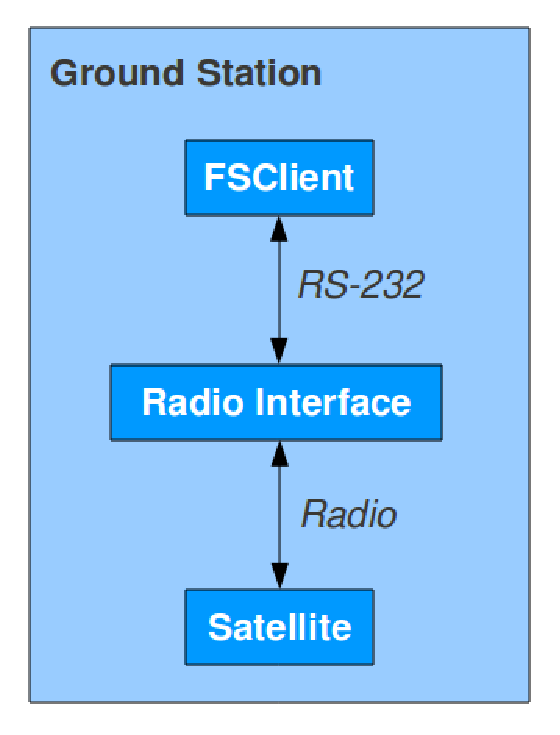
\includegraphics[scale=0.5]{img/interaction_via_console}
  \caption{FSClient on the Ground Station}
\end{figure}

\subsection{GUI}
There are many posibilities when it comes to implementing a GUI but regardless of the choice there must be communication with the satellite over the radio.

One way to solve this is to let the GUI connect to the Ground Station via SSH and use fsclient each time it must send a failsafe request.

A drawback to this solution is that not all GUI frameworks and operating systems have support for SSH out of the box.

\subsection{TCP Interface to the radio}
Alternatively there could be a TCP server on the Ground Station that listens for failsafe commands from connected TCP clients and have them forwarded to the radio. With this TCP server, called fsserver, we effectively have a TCP interface to the satellite and the advantage here is that all major GUI frameworks and all major operating systems have TCP support making this solution far more flexible than the SSH solution.

\begin{figure}[h!] \centering
	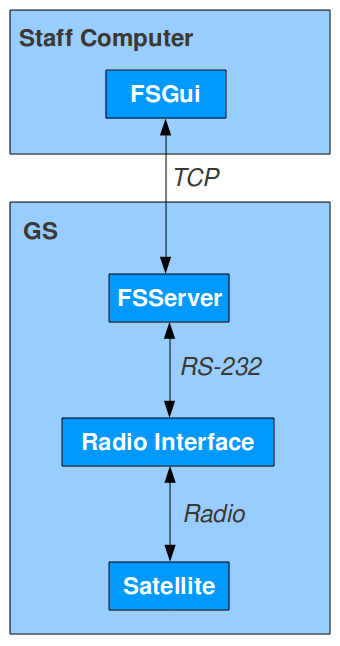
\includegraphics[scale=0.5]{img/tcp_interface_to_the_radio}
  \caption{TCP Interface to the radio}
\end{figure}

\subsection{Command Combinations}
The failsafe software has a set of basic commands which by themselves are of limited use but becomes powerful when combined. As we cannot know which failures might occur in the future, it is critical that there is a flexible way of combining these commands in conditionals and loops.

One solution is to combine the commands in the GUI. Then we would need to construct individual GUI elements for concepts like a command, a command sequence, an if statement and its branches, a loop statement and its body and so forth. This solution is hard to extend with a switch-statement in two years time when someone needs it - and impossible to do without the source code.

The use of script languages to combine commands
Alternatively there is a far more flexible solution to this challenge when it is recognized that conditionals and loops already have been implemented numerous times in script languages such as Ruby, Python or TCL and that they can be used to achieve the required flexibility.

Send failsafe commands from a script using UNIX
It is necessary that the scripts can communicate with the Ground Station. To solve this each script could implement a TCP client, but that would mean two things. One, a TCP client for each specific language would be needed before they could be used to write failsafe scripts. This is inflexible. Two, there would exist several implementation of the TCP client which is error-prone.

Is there anything all scripting languages have in common? Well, if we assume that the scripts are being run on a UNIX system, they will have exactly that in common. All languages have built-in libraries for running a UNIX console command and manipulating the output. So, we could use fsclient to pass failsafe commands through. Fsclient will just handle the TCP connection to the Ground Station and forward the commands.

FSServer must be aware of multiple TCP clients and ensure that commands from various TCP clients are not executed at the same time. This challenge is covered the chapter \ref{chap:fsserver}.

\begin{figure}[h!] \centering
	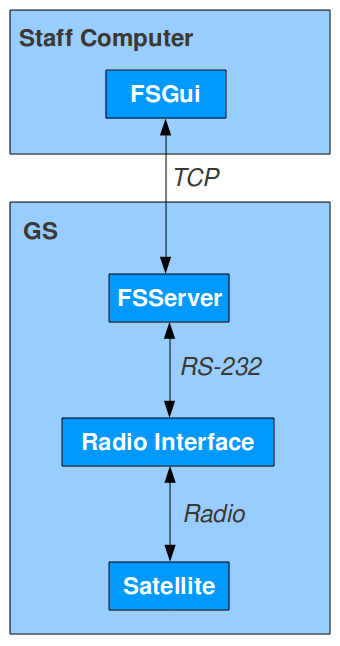
\includegraphics[scale=0.5]{img/tcp_interface_to_the_radio}
  \caption{FSClient and executing scripts}
\end{figure}

\subsection{Graphical representation of the health status}
The failsafe software has a command called HEALTH\_STATUS which will return a set of numbers representing the state of the subsystems. These numbers will be interpreted as temperature, current and voltage values in the GUI. The GUI must provide a graphical representation of the subsystems and their health status.

\section{Chosen design}
Here is a wrap up of the final design that consists of four key elements:

\textbf{FSServer}
\begin{itemize}
	\item Installed on GS
	\item A TCP server
	\item Send failsafe commands via the datalink
	\item Send failsafe response back to TCP clients
	\item Ensure atomicity of failsafe commands
\end{itemize}

\textbf{FSClient}
\begin{itemize}
	\item Installed on the staff's desktop computers
	\item Unix program
	\item A TCP client to FSServer
	\item Forward failsafe commands from other unix programs to the server
	\item Interactive mode
\end{itemize}

\textbf{FSGui}
\begin{itemize}
	\item Installed on the staff's desktop computers
	\item Runs on unix and windows systems
	\item A TCP client to FSServer
	\item No installation required, just download and double-clik
	\item Create, save, load, export command sequences
	\item Execute failsafe scritps
	\item View graphical representation of the health status
\end{itemize}

\textbf{Scripts}
\begin{itemize}
	\item Any script or programming language that can execute unix commands
	\item Combine failsafe commands in conditionals and loops
\end{itemize}

\begin{figure}[h!] \centering
	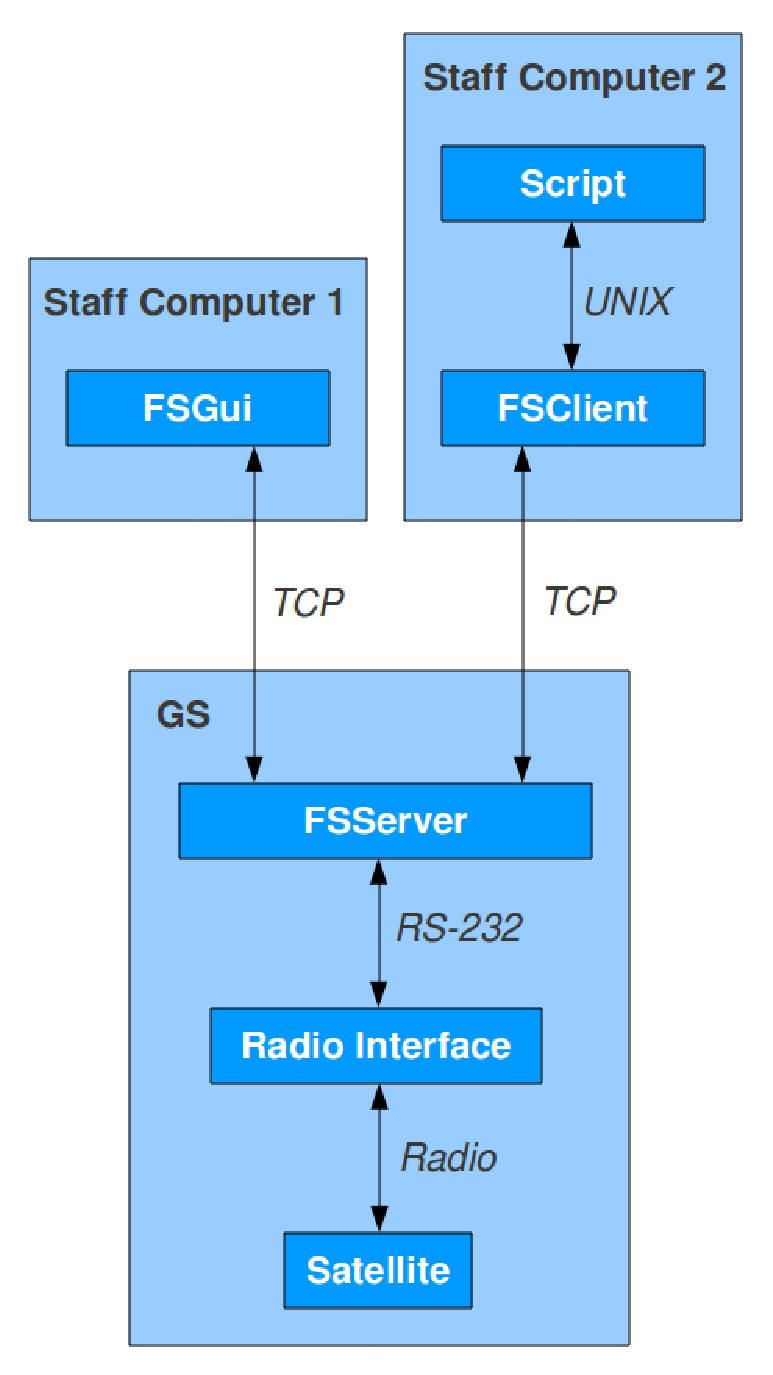
\includegraphics[scale=0.5]{img/chosen_design}
  \caption{The chosen design}
\end{figure}

Now that there is an overall design, lets proceed with an analysis, design and implementation part of the individual parts.

%\chapter{FSServer}
\label{chap:fsserver}
This chapter deals with the requirements specification, analysis, design and non-trivial implementation details of FSServer.

\section{Requirements Specification}

The requirements for FSServer are:

\begin{itemize}
	\item must be installed on GS
	\item must accept TCP connection
	\item must send failsafe commands via the datalink
	\item must send failsafe responses back to TCP clients
	\item must ensure atomicity of failsafe commands
\end{itemize}

In addition to these requirements, the following requirements was identified when the overall design was agreed upon:

\begin{itemize}
	\item must run as a daemon and log all activity to a file
	\item must execute scripts on GS and from a TCP client and immediately send any response back to the TCP client
	\item must validate failsafe commands
\end{itemize}









\section{Analysis and design}
Lets go through the requirements one by one. For each requirement we will enhance the design to incorporate the requirement.

\textbf{Must be installed on GS} \\
Trivial constraint.

\textbf{Must accept TCP connections} \\
Clients can connect to the server with the TCP protocol over an internet socket.
The server could accept one or multiple connections at a time. We want to ensure that only one command is send to the satellite at a time, so lets accept only one connection for now.

\textbf{Must send failsafe commands via the datalink and send response back to clients} \\
We could implement pull-behaviour where each request is answered with exactly one response or we could implement push-behaviour where data can be pushed to the client without being requested. It is not obvious which of these behaviours we should implement so lets choose the pull-behaviour for now.

\textbf{Must ensure atomicity of failsafe commands} \\
Only one satellite command can be executed at a time. If we use a request queue with atomic enqueue and dequeue operations we can implement this behaviour without race conditions.

\textbf{Must run as a daemon and log all activity to a file} \\
A unix daemon is a process with a parent process id of 1. When starting the server, the staff must be able to decide whether to run it as a daemon or to run it as a normal process.
The logfile could be a predefined file, but we should let the staff decide by providing an option when starting the server.

\textbf{Must execute scripts on GS and from a TCP client and send any response back to the TCP client} \\
Some tasks, such as uploading a binary file to the satellite, are so common that they should be available for every client. Instead of implementing these tasks in every client, the server should implement them and execute them when requested by the client.
The scripts can be written in any language that is supported by the server environment. To capture the output of a script, the server will open a pseudo terminal that has control of standard output and input. The script is executed in the pseudo terminal and any output can be send to the client.

\textbf{One or multiple TCP connection} \\
Now consider the following scenario. A client connects to the server and requests to execute script X. Because of the pull behaviour we decided upon earlier the client will now wait for the script to finish with the response. If script X needs to interact with the satellite, it must connect to the server and do some requests but the server only accepts one TCP connection at a time, and we have a deadlock situation.

\begin{figure}[h!] \centering
	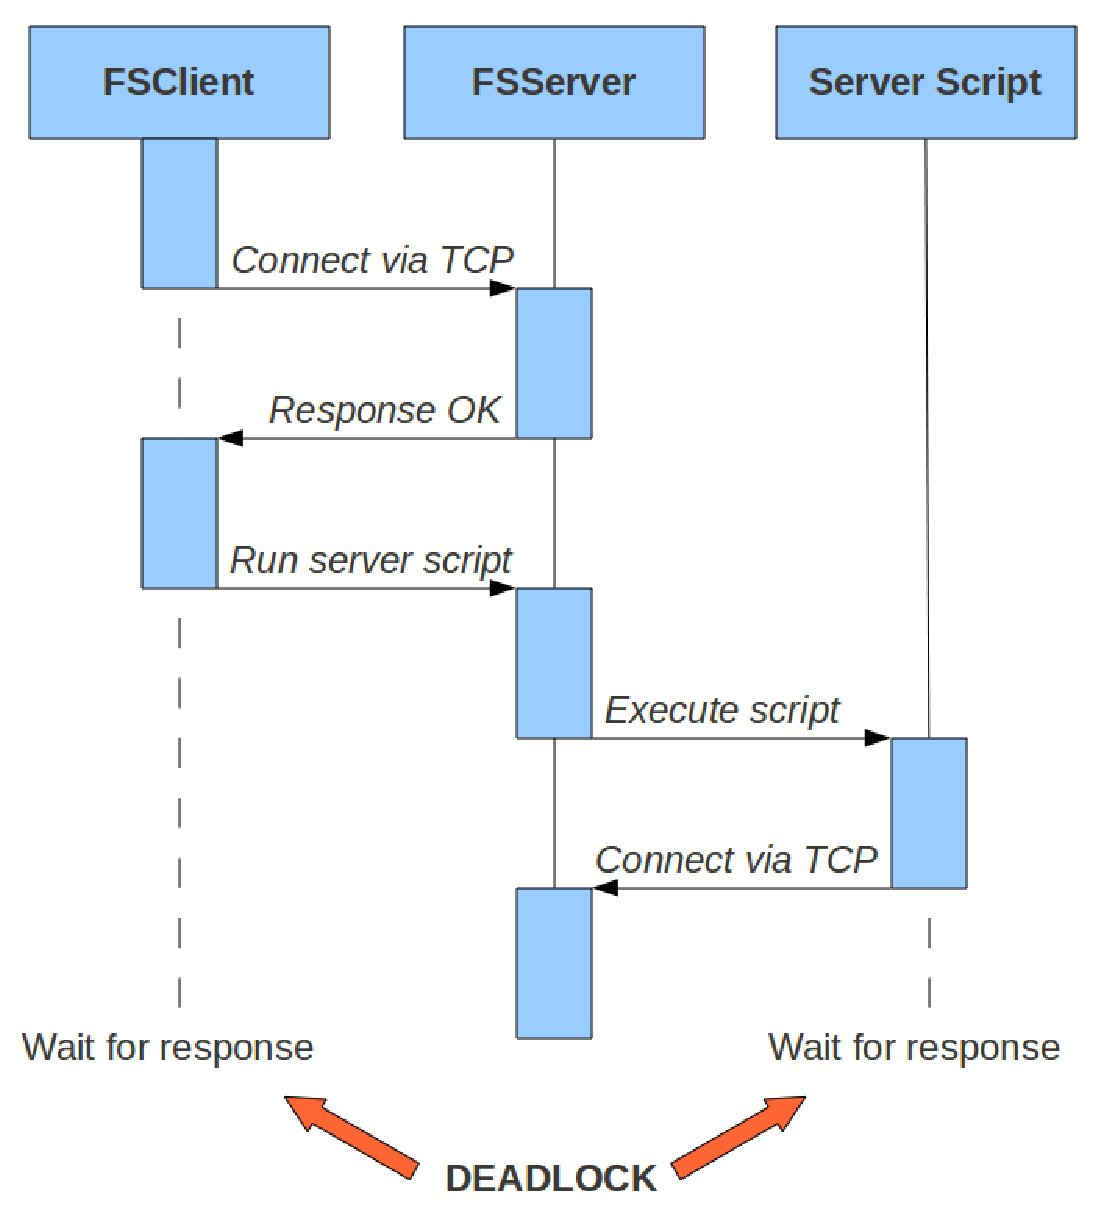
\includegraphics[scale=0.5]{img/one_connection_deadlock}
  \caption{Deadlock when executing script}
\end{figure}

So there is a need for handling multiple TCP clients and their requests simultaneously. Satellite commands over the serial connection must not be simultaneous however!

\textbf{Blocking vs. non-blocking execution} \\
In a program a non-blocking execution of a statement will not wait for the result of that statement before proceeding with the execution of the next statement. A blocking execution of a statement will wait for the result before proceeding.
In order to handle multiple TCP clients concurrently the server must execute the requests in a non-blocking fashion.

\textbf{Lock mechanism} \\
With multiple clients new concerns must be dealt with. Consider the scenario where two clients execute a server script each. The script consists of 2 satellite commands and although we can ensure that only one satellite command are being executed at a time, we can not ensure that the 2 commands are executed sequentially.

\begin{figure}[h!] \centering
	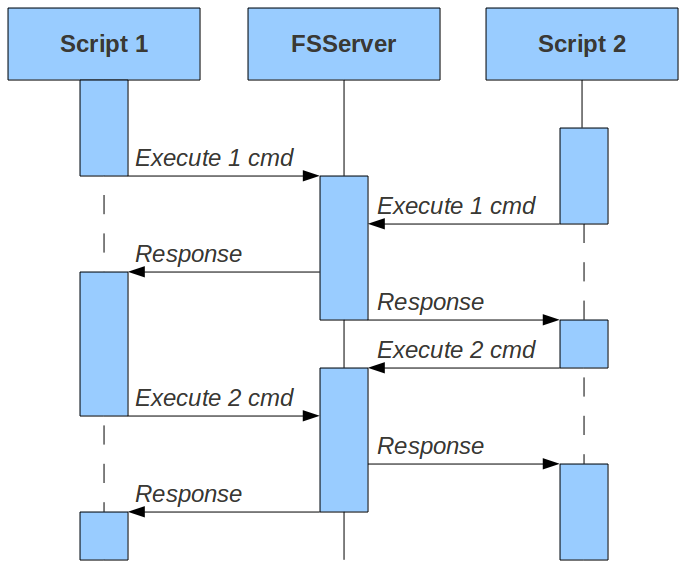
\includegraphics[scale=0.5]{img/multiple_scripts_no_lock}
  \caption{Two scripts executing without locking}
\end{figure}

We need a way to lock the server to prevent multiple executing scripts from stepping on each others toes. So after connecting to the server a client must first issue a lock request and will receive a session token if the lock succeeded or a message indicating that the server is already locked.

When finished an unlock request can be sent to unlock the server. Things can go wrong however and leave the server in a locked state, so there will be implemented a timeout on the token. After each request this timeout will be reset. If the token gets timed out, a broadcast message will be sent to all connected clients.
It is important to note that two scripts requested by clients using the same token will be executed simultaneously!

\begin{figure}[h!] \centering
	
\includegraphics[scale=0.5]{img/lock}
  \caption{Two scripts executing with locking}
\end{figure}

\textbf{Partial responses} \\
Another thing to consider is the output of the server scripts. Imagine for instance an upload script that prints to standard out each time 10\% of the upload is done. The client would like to follow this progress in real time as opposed to seeing the total output of a script when execution has finished. So in the case of the upload script we would at least be sending 10 partial messages in response to one request.
This along with the timeout broadcast leads to the need for pushing data to clients and we must therefore implement the push-behaviour in favor of the pull-behaviour.

\begin{figure}[h!] \centering
	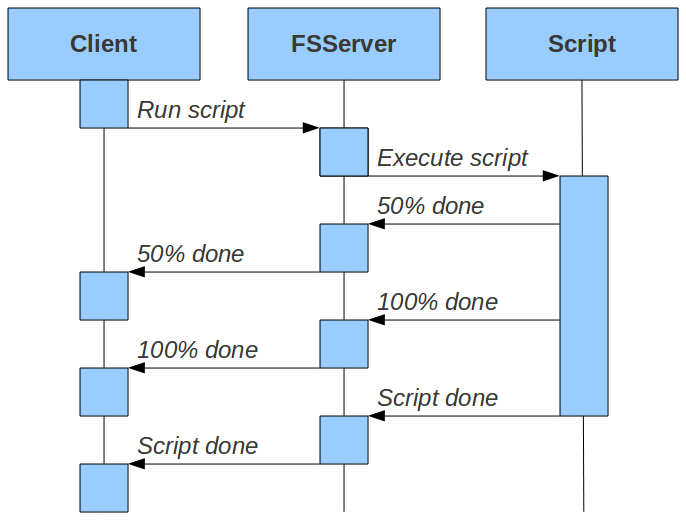
\includegraphics[scale=0.5]{img/partial_responses}
  \caption{Partial response}
\end{figure}

\textbf{Must validate failsafe commands} \\
Failsafe commands can have arguments such as "address", "length" etc. These arguments must be validated before being send to the satellite. Arguments are typically memory addresses and other hexadecimal values. It would be convenient to use both hexadecimal ("0xff") and decimal ("255") values as arguments. If an argument is invalid or missing the client must be informed and the request must not be executed.

\subsection{Data format}
Now that we have a design that covers all features, lets look at the data format. We have several choices here. We could go with a simple text format, XML or JSON.

The client must be able to send a message to the server and react to the received response. There must be a way of determining whether incoming data is a response to some outgoing data. As there are no such information in the order of the outgoing and the incoming data, a request must be stamped with a unique identification key that can be used by the server to stamp the response. The data format must at least have two parameters then, a stamp and the data.

If we use a simple text format we would need a separator to distinguish the parameters. Then we would have to care about escaping certain characters etc. Instead we should consider using the semantically equal XML or JSON formats. We will be using JSON.

\begin{itemize}
	\item Request: \texttt{\{"id":KEY, "data":REQUEST\}}
	\item Response: \texttt{\{"id":KEY, "data":RESPONSE\}}
\end{itemize}
Example of a "lock" request:
\begin{itemize}
	\item Request: \texttt{\{"id":"1","data":"lock"\}}
	\item Response: \texttt{\{"id":"1","data":"7KFdnNXBYi8nmuWV"\}}
\end{itemize}

If the client has locked the server, the token is sent along the request like this:

\begin{itemize}
	\item Request: \texttt{\{"id":"1","data":"reset","token":"7KFd"\}}
\end{itemize}

Besides from being able to respond to incoming requests, the server also needs to push data to the client independently of any requests. The client must be able to determine the data type to handle it correctly. The format must at least look like:

\begin{itemize}
	\item Message: \texttt{\{"type":TYPE\}}
\end{itemize}

Example of an "token timout" message:

\begin{itemize}
	\item Message: \texttt{\{"type":"server\_unlocked"\}}
\end{itemize}

For format consistency and faster processing on the client side, the response format will also have the type parameter:

\begin{itemize}
	\item Response: \texttt{\{"type":"response", "id":KEY,"data":RESPONSE\}}
\end{itemize}

The server must also be able to send more than one response to a given request. This can be solved with the following format:

\begin{enumerate}
	\item Req: \texttt{\{"id":"2", "data":"run\_script upload filepath", "token":"7KFd"\}}
	\item Res: \texttt{\{"type":"response", "id":"2", "data":"50\% done", "partial":"true"\}}
	\item Res: \texttt{\{"type":"response", "id":"2", "data":"100\% done", "partial":"true"\}}
	\item Res: \texttt{\{"type":"response", "id":"2", "data":""\}}
\end{enumerate}

























\section{Implementation}
This section deals with the non-trivial implementation details.

\textbf{Language and libraries} \\
There are no contraints to the programming language and as the server will neither be cpu- or io intensive the server has been implemented in Ruby. It could have been implemented in C or Java, and probably should have if there where any requirements to speed.

Ruby has a standard library with support for basic things like sockets, threads, system etc. There is a packaging tool called rubygems with which one can install third party libraries called gems.

Instead of reinventing a TCP server, a serialport wrapper and a JSON parser we will be using production ready ruby gems that has been tested over long periods of time by many people and have been accepted within the ruby community.

Third-party gems used in the implementation:
\begin{itemize}
	\item \textbf{Eventmachine} - Instead of the relatively slow socket support in the standard library we will be using the evetnmachine gem. Eventmachine is a library for implementing non-blocking TCP servers and clients.
	\item \textbf{JSON} - provides a JSON parser class.
	\item \textbf{Serialport} - provides a class for using RS-232 serial ports.
	\item \textbf{Daemons} - provides an easy way to wrap existing ruby scripts to be run as a daemon and to be controlled by simple start/stop/restart commands.
\end{itemize}



\textbf{Safe script execution} \\
When executing server scripts from a client we must be very careful about the parameters. Consider the scenario were a client sends this request:
\begin{verbatim}
	run_script scriptname param1;rm -rf}
\end{verbatim}
If we are not careful and just pass along the parameters without escaping the semicolon, the result of this command will delete all files on the server, that the currently running user has permissions for.

Ruby has a wrapper for the UNIX command execve. Execve can create new UNIX processes and will safely pass arguments along.
Ruby's pseudo tty library uses the execve wrapper to execute console commands.

\textbf{Failsafe Commands} \\
A failsafe command is a Ruby class that can have an initialize, a validate and an execute method. Initialize takes the arguments for the command, validate will validate the arguments and execute will execute the command.

All commands inherits common code from the AbstractCommand class. This class implements some common validations, a default initialize method, a default validate method and a default execute method.

\textbf{Parsing} \\
When the server gets a new request, it is parsed with the JSON gem. The id and token are easily looked up in the resulting Ruby hash. The data field is first split on spaces to separate the command from its arguments. The command is then camelized which means that the first character and any characters immediately after an underscore is capitalized. The underscores are then removed. Each command has a corresponding camelized Ruby class.

For example: \\
The server receives this request:
\begin{verbatim}
	{"id":"1","token":"abcdefg", "data":"run_script filepath arg1 arg2"}
\end{verbatim}

First it is parsed as JSON. This results in a Ruby hash where we immediately lookup the id and the token. The data is then split on spaces:

\begin{verbatim}
	cmd, *arguments = parsed_request["data"].split
\end{verbatim}

Ruby has a function called eval that takes a string as a parameter and executes that string as Ruby code. To get an instance of the camelized class to a run\_script command we can execute the following:

\begin{verbatim}
	eval(cmd.camelize+".new(*arguments)")
\end{verbatim}

which is equivalent to:

\begin{verbatim}
	eval("RunScript.new(*arguments)")
\end{verbatim}

When this string is executed by eval, the initialization code for RunScript will be called with all the arguments.

Options are also extracted. If an argument begins with a dash ("-") then it will be split on equal-signs and stored in an options hash.

Again we must be very careful when executing a string from an unknown place. In this way a user could create an instance of any Ruby class and pass any arguments to it. To deal with this, we encapsulate all valid commands in a module called Commands. So now the eval looks like:

\begin{verbatim}
	eval("Commands::#{cmd.camelize}.new(*arguments)")
\end{verbatim}

\textbf{Validation} \\
When the command has been parsed the server will call the validate method before calling the execute method. If the validate method fails the execute method will never be called, instead a failed validation message is sent to the client.

Common validations are implemented in the AbstractCommand class and uses some extensions to the String class. The most common validation is to ensure that the argument is addressable. To be addressable the value must be given as a hex or a decimal value. The validation ensures that the value is not greater than 0xffffffff.

\textbf{Satellite IO} \\
The server will have to communicate with the radio link on GS when communicating with the satellite. During development however a development board has been used. This board has a RS-232 interface, so the serialport gem has been used to write an serialport implementation that adheres to the protocol layer interface.

\textbf{Request queue with atomic enqueue and dequeue operations} \\
It is important that only one command is being sent at any given time to the satellite. Therefore, a ProcessingQueue module has been implemented. A processing queue has an array of requests, a mutex and a boolean value to indicate that the processing has already started. When enqueueing, the request is put into the queue when the mutex becomes available. Then the processesing loop is started unless it has already been started.

The queue is when the mutex becomes available and the request is processed. As soon as the processing is done the mutex is released and the processing is started again until there is no more requests left in the queue.

Option for satellite commands:
\begin{itemize}
	\item \textbf{--timeout=SEC} - There is a timeout for each executing satellite command. It is set to 5 seconds by default but can be changed per request with the timeout options e.g. "reset" and "reset --timeout=20" are both valid commands. The former will timeout after 5 seconds and the latter will timout after 20 seconds.
	\item \textbf{--no-response} - Sometimes we do not care about the response for a command and would like to skip it in order to save execution time and batterylife. The option looks like this: "reset -no-response".
\end{itemize}

\textbf{Broadcasting} \\
Broadcasting can be done by maintaining a global array of connected clients. A message can then be sent to each client.

\textbf{Token handling and timeout} \\
The TokenHandler class is responsible for timing out the token. It has a token variable, which is just a string. The server is unlocked if this value is nil. When setting the token variable a timer will be started. If the timer runs out the token variable will be set to nil and a broadcast message is sent to all connected clients.

\textbf{Logging} \\
When starting the server one can indicate to use a logfile for the server output. If none is indicated the server will print its output to standard out.

%\chapter{FSGui}
\label{chap:fsgui}
This chapter will deal with the requirements specification, analysis, design and non-trivial implementation details of FSGui.

\section{Requirements Specification}
The requirements for FSGui are:
\begin{itemize}
	\item must be installed on the staff's desktop computers
	\item must run on unix and windows systems
	\item must be a TCP client to FSServer
	\item must not need installation, just download and double-clik
	\item must create, save, load, export command sequences
	\item must execute failsafe scritps
	\item must view graphical representation of the health status
\end{itemize}
In addition to these requirements, the following requirement was identified when the overall design was agreed upon:
\begin{itemize}
	\item must be able to retrieve a list of server scripts and execute them with custom arguments
	\item must be able to execute local scripts
	\item must have an auto\_lock option
	\item must indicate connection and lock state
\end{itemize}

\section{Analysis and design}
Lets go through the requirements one by one. For each requirement we will enhance the design to incorporate the requirement.

\textbf{Must be installed on the staff's desktop computers} \\
Trivial constraint

\textbf{Must run on unix and windows systems} \\
There exists a number of cross-platform GUI frameworks we could use like Java swing or Xulrunner.

Xulrunner is Mozilla's cross-platform and open source framework. Xulrunner has the advantage that it is very easy to build complex and appealing GUIs in no time. The disadvantage is that the framework takes up 20 MB of harddisk space and is not included on UNIX og Windows by default. Furthermore, it lacks some systemwise features like spawning new processes and executing console commands.

The advantage with Java is that it runs on most systems and once you have the java virtual machine installed it is fairly easy to just pack an executable jar file and run it with a double click.
The FSGui will be implemented in JAVA using the Swing Framework.

\textbf{Must be a TCP client to FSServer} \\
When the program starts the user must indicate the address and port of the FSServer.
With a 30 sec token timeout the user will experience lock errors often enough to be annoying. Therefore, it must be possible to set an autolock option. It must also be clear to the user whether the server is locked or not and whether a connection has been made to FSServer or not.

\begin{figure}[h!] \centering
	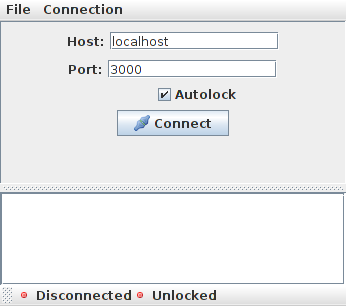
\includegraphics[scale=0.5]{img/fsgui_connect}
  \caption{The connect panel}
\end{figure}

\textbf{Must not need installation, just download and double-clik} \\
The FSGui will be packed as an executable jar file. The only requirement to the staff computers is that they have a Java Virtual Machine installed.

\textbf{Must send failsafe commands} \\
Java has built-in support for sockets and TCP.

\textbf{Must create, save, load and export command sequences} \\
For easy and fast testing, simple command sequences can be composed in the GUI. There are no conditionals or loops and the sequence will stop executing if one of the commands fails for one reason or another. It is possible to save and load sequences and to export a sequence to a Ruby script.

Sequences can be saved, loaded and exported to scripts.

\begin{figure}[h!] \centering
	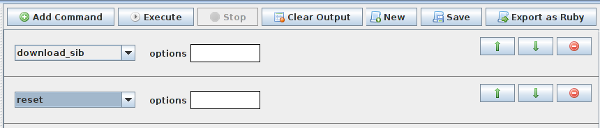
\includegraphics[scale=0.5]{img/fsgui_sequences}
  \caption{Command Sequences}
\end{figure}

\textbf{Must view graphical representation of the health status} \\
The satellite can read various health information from the individual subsystems and send them back to earth. Which data the subsystems will actually yield and how that data should be interpreted is not agreed upon as of this writing.

Instead the development board, that was used in place of the real satellite, simulates this data by reading several voltages and currents. When the real data is available the staff should be able to modify the source code of this project and fairly quickly replace the development data with the real data.

\begin{figure}[h!] \centering
	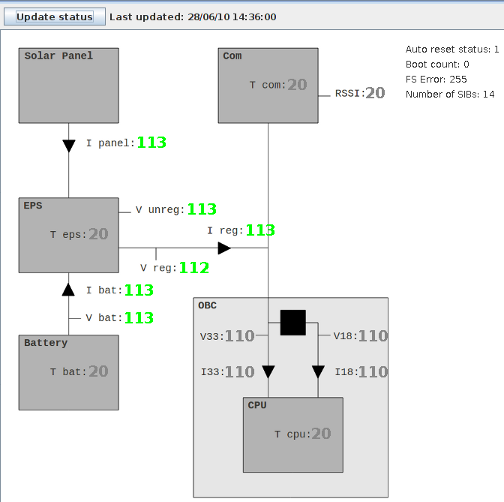
\includegraphics[scale=0.5]{img/fsgui_health}
  \caption{The Health Status}
\end{figure}

\textbf{Must be able to execute local scripts} \\
In addition to running a script in the console it should also be possible to run and see the output of that script from within the GUI. The scripts are organized in a filetree and the user should be able to set the root of the filetree, navigate through the filetree, selecting a script, passing arguments to it and executing it.

\begin{figure}[h!] \centering
	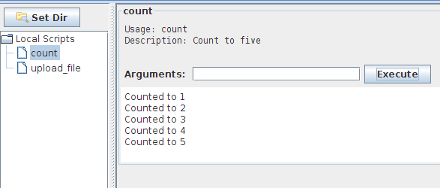
\includegraphics[scale=0.5]{img/fsgui_local}
  \caption{Local Scripts}
\end{figure}

\textbf{Must be able to retrieve a list of server scripts and execute them with custom arguments} \\
FSGui can retrieve a list of available server scripts that the user can choose from. FSServer will implement the available\_scripts command to retreive this information. Once retrieved the GUI builds a tree of the scripts for easy navigation.

When a script has been clicked on in the tree, a script description and a textfield for passing arguments are presented to the user. An execute button will execute the script on the server, any response data will be appended just below the script.

\begin{figure}[h!] \centering
	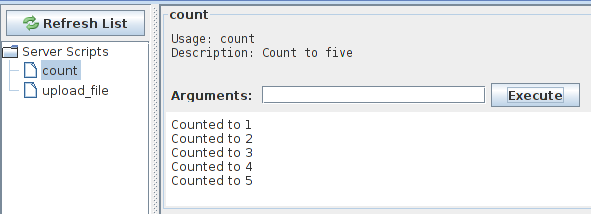
\includegraphics[scale=0.5]{img/fsgui_server}
  \caption{Server Scripts}
\end{figure}

\textbf{Must have an auto\_lock option} \\
An auto\_lock option is available in the connect panel and from the menubar.

\begin{figure}[h!] \centering
	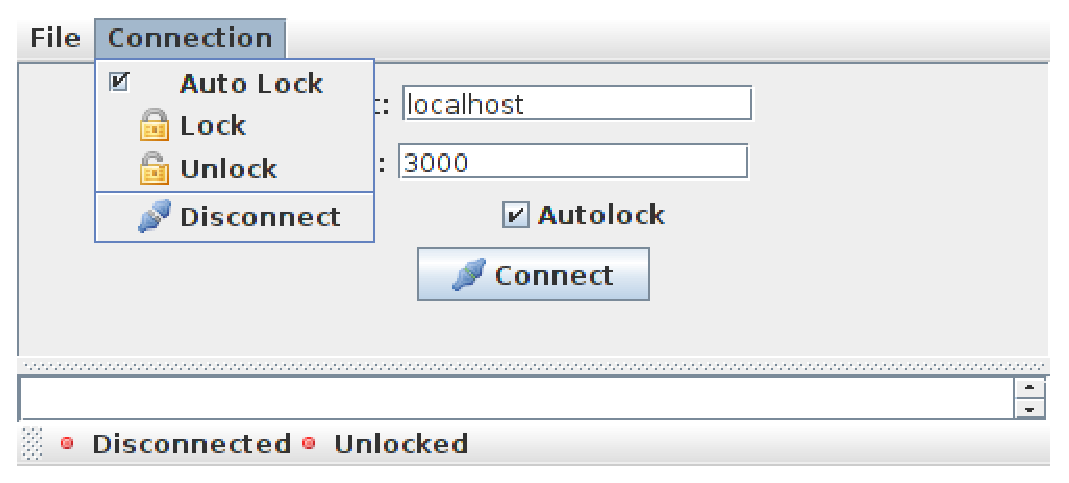
\includegraphics[scale=0.5]{img/fsgui_autolock}
  \caption{Auto Lock, connection and lock status}
\end{figure}

\textbf{Must indicate connection and lock state} \\
There is a statusbar in bottom of the window indicating whether there is a connection or not and whether the server is locked by the gui or not.










\section{Implementation}
Lets look at the non-trivial part of the implementation.

\textbf{FSController} \\
At the heart of the FSGui is the FSController singleton class which is responsible for creating the TCP socket, building the swing gui and setting up the data handlers. Because of its bigbrother like nature it is also extensively used in other classes to reference other parts of the program.

\textbf{Local Scripts} \\
Java has a built-in class called ProcessBuilder that can create a process given a list of the command and its arguments. It will execute and capture the output of the process. We will use this class to execute local scripts.

\textbf{Socket and Socket Callbacks} \\
The built-in class Socket will be used to create the TCP connection and to read/write on the socket. To prevent cluttering in FSController the Socket will be wrapped in a class called FSSocket that will perform callbacks to a class that implements the FSSocketObserver interface when interesting events happen, such as on connection, on disconnection, on incomming data etc. The FSController implements this interface and will therefore be able to act on these events.

\textbf{Data Handlers and request callbacks} \\
When we send a request to the server we will often expect some kind of response. As the solution is push driven we cannot know when the response will come. We cannot send the request and then immediately wait for the response on the socket, potentially throwing away responses to other requests. We have to send the request and just hope that the response will come.

When the response finally do come, we won't know what to do with it. So along with sending a request we most associate it with a callback that should be executed upon a received response.

This is done with a FSCallback which is an interface consisting of one method called onResponse that takes a FSResponse as its parameter. The callback is registered in the requestCallbacks Hashtable where an entriy consists of the requests id as key and the callback as a value.

A class called FSSocketReader will constantly be reading the socket and whenever a message has been read it is first sent to the appropriate data handler and if it is a response, the response handler will look for the id in the requestCallbacks and execute the callback.

When the client gets an incoming message FSGui determines the type of the message and dispatches it to the appropriate data handler. Data handlers must therefore be setup before connecting to the server.

\textbf{The response handler} \\
When sending a request one specifies what piece of code to run when the response is received.
The response handler looks at the id parameter and matches it to the corresponding request and dispatches the data to that piece of code.

\textbf{The token timeout handler} \\
This handler just notifies the user by changing the "locked"-icon in the GUI.

\textbf{JSON Parsing} \\
Java does not have built-in support for JSON, so a third-party library called JSONObject has been used.

\textbf{Generating unique ids for the requests} \\
Unique id generation is handled by FSSocket and is appended the the request before sending it off to the server. It is a fairly simple algorithm that uses Java's builtin SecureRandom and BigInteger classes. The produced id is a 5 digit integer. The odds of two requests having the same id is 1 to 10000 which is assumed to be acceptable.

\textbf{Command Sequences} \\
The command sequences are saved in a simple json format. A sequence of the following commands:
\begin{verbatim}
	health_status
	download 0x40000000 512
\end{verbatim}
Will be saved as the following JSON data:
\begin{verbatim}
[
	{"command":"health_status", "arguments":[""]},
	{"command":"download","arguments":["0x40000000","512",""]}
]
\end{verbatim}
NOTE: The empty string in the end of each argument is the options textfield.

%\chapter{FSClient}
\label{chap:fsclient}

This chapter will deal with the requirements specification, analysis, design and non-trivial implementation details of FSClient.

\section{Requirements Specification}
The requirements for FSClient are:
\begin{itemize}
	\item must be installed on the staff's desktop computers
	\item must be a unix program
	\item must be a TCP client to FSServer
	\item must forward failsafe commands from other unix scripts to the server
	\item must have an interactive mode
\end{itemize}
In addition to these requirements, the following requirements was identified when the overall design was agreed upon:
\begin{itemize}
	\item must have a data\_only mode
	\item must have an auto\_lock mode
\end{itemize}

\subsection{Analysis and design}
Lets go through the requirements one by one. For each requirement we will enhance the design to incorporate the requirement.

\textbf{Must be installed on the staff's desktop computers} \\
Trivial constraint.

\textbf{Must be a unix program} \\
Trivial constraint.

\textbf{Must be a TCP client to FSServer} \\
Trivial constraint

\textbf{Must forward failsafe commands from other unix scripts to the server} \\
Fsclient will take a failsafe command and its arguments as parameters, send it over TCP to the server and print the response to standard out.

\textbf{Must have an interactive mode} \\
In interactive mode, it prompts the user for a failsafe command, sends it to the server, retreives the response, prints the response and prompts the user again until the user enters exit. The --interactive option will do this.

\textbf{Must have a data\_only option} \\
Sometimes we don't want to see the entire response message but just the data field. The \texttt{--data-only} option will do this.

\textbf{Must have an auto\_lock option} \\
There should also be an option for auto locking when starting the interactive mode. The \texttt{--auto-lock} option will do this.

\subsection{Implementation}
This section deals with the non-trivial implementation details.

There are no contraints to program speed so the FSClient has been implemented in ruby.
Fsclient uses rubys standard command "\$stdin.gets" to prompt the user for input.
The TCP connection has been implemented with eventmachine.

%\chapter{Upload File Script - an example of a user script}
\label{chap:upload_script}
This chapter analyses the requirements and discuss various design alternatives of the upload script. The implementation details of the chosen design will follow.

\section{Analysis and Design}

The upload file is an example of a user script. It must take a filepath as parameters and upload it to the flash on the satellite. There are no failsafe command to upload a file to the flash, so a script must written that uses several failsafe commands to achieve to overall goal.

Firstly the script must be divide the file in parts of the maximum data size and upload them to the satellite ram memory. After uploading to ram it must copy the data from the ram to the flash and lastly calculate the checksums to ensure that everything got copied correctly.

The staff typically wants to upload a new version of the nominal mode. There are different ways of storing the nominal mode in a file. It can be stored as binary data in a file or as hex formatted data in a file.

This script will assume that the data is stored as a binary file. Therefore addresses to the ram and flash memory must also be given as arguments.

During upload the user must be notified with the overall progress.

\section{Implementation}
The script is an executable file written in ruby with the following path \texttt{"scripts/upload\_file"}.

It takes three arguments: token, filepath and ram\_address flash\_address.

It validates that these three arguments have been given, that the file exists and that the address is a valid address.

Then it determines the size of the file, and how many individual uploads there is needed to upload the entire file.

For each upload the bytes to be uploaded are read from the file and uploaded via fsclient.

The progress is printed.

If the upload went well the next part of the file will be uploaded.

If the upload went bad the script is stopped and the user is notified.

When the upload has finished it will start the copying from ram to flash.

When the copying is done the checksum will be calculated to ensure that everything is OK.

\textbf{Maximum data size of 20 bytes} \\
The upload script has a maximum data size of 20 B instead of the allowed 1020 B. This is because the current implementation of the failsafe software has some problems with data being send too fast. The current workaround is to sleep for 0.2 seconds inbetween each byte written. It will takes 204 seconds to upload 1020 bytes and in that time space the satellite will reset and the command will fail. In contrast it takes 4 seconds to upload 20 bytes.

The maxumum data size should be changed when the issue has been fixed in the failsafe software.

%\chapter{Tests and Results}
\label{chap:test}
Now that the implementation is complete, we should test that it meets the requirements of the system and ultimately give us an idea of the success of the project.

This chapter will start by stating the test stragedy. Then the test setup is described along with an example of a test case. Then all test cases are outlined. The chapter ends with a summary of the test results.

All test cases can be found in Appendix \ref{appendix:C}.

\section{Test Stragedy}
The stragedy has been to perform functional tests of all requirements. The tests are combined in integration tests as some requirements span over the individual subsystems.

Unit tests have been performed on the command validations.

Lastly all failsafe commands have been tested with fsclient.

\section{Test Setup}
The setup has consisted of two, sometimes three, terminals. FSServer ran in the first terminal logging to standard out. Commands was then send via FSClient in the other terminals and the outcome of the test was determined based on the response and log messages of FSServer.

Unit tests was implemented in ruby with the built-in UnitTest library. To run the validation tests for example type \texttt{ruby test/lib/string\_test.rb}

\section{List of Test Cases}
The test cases all follow the same format:

	ACTION, EXPECTED, RESULT

If it makes sense a test case will have more data. For example, a failsafe command test case also states what has been written and read on the datalink:

\begin{center}
    \begin{tabular}{ | p{3cm} | l |}
    \hline

		\textbf{FSClient args} & \texttt{calculate\_check\_sum 0 128} \\ \hline
		\textbf{Datalyer write} & \texttt{0a 00 08 00 00 00 00 00 80 00 00 00 CD} \\ \hline
		\textbf{Expected} & Return code = \texttt{0x0a} \\ \hline
		\textbf{Datalayer read} & \texttt{0a ff 04 00 15 04 92 a7} \\ \hline
		\textbf{Response} & \texttt{\{"status":10,"data":2811364373,"message":"ACK"\}} \\ \hline
		\textbf{Result} & \texttt{success} \\ \hline

    \end{tabular}
\end{center}


Here is a list of all the test cases:
\begin{itemize}
	\item FSServer

	\begin{itemize}
		\item Daemonization
		\item Custom logfile
		\item Multiple tcp clients, lock mechanism, token timeout, no-response and broadcast
		\item Command parsing
		\item Sequentially executed satellite commands
		\item Command validation
		\item Spaced hex
	\end{itemize}

	\item Commands
		\begin{itemize}
			\item Calculate Check Sum
			\item Call Function
			\item Copy To Flash
			\item Copy To Ram
			\item Delete Flash Block
			\item Download
			\item Download Sib
			\item Execute
			\item Flash Test
			\item Health Status
			\item List Scripts
			\item Lock
			\item Ram Test
			\item Read register
			\item Read sensor
			\item Reset
			\item Reset Sib
			\item Run Script
			\item Set Autoreset
			\item Sleep
			\item Unlock
			\item Unlock Flash
			\item Upload
			\item Upload Sib
			\item Write Register
		\end{itemize}

	\item FSGui
	\item FSClient
	\item Upload File Script

\end{itemize}

\section{Test summary}
This section will summarize the test results.

\textbf{FSServer test results} \\
All integration tests passed. \\
All unit tests passed. \\
All but 3 command tests passed:
\begin{itemize}
	\item \textbf{Flash Test} - Does not return a test result in the data.
	\item \textbf{Health Status} - 20 bytes is read from the datalink instead of 16 bytes.
	\item \textbf{Upload Sib} - Flash Write Error when uploading a new sib
\end{itemize}
FSServer works as expected and according to the requirements, the failsafe commands flash\_test, health\_status and upload\_sib do not however.

\textbf{FSGUI test results} \\
All tests passed.\\
FSGui works as expected and according to the requirements

\textbf{FSClient test results} \\
All tests passed.\\
Fsclient works as expected and according to the requirements

\textbf{Upload File Script test results} \\
All tests passed.\\
The upload scripts works as expected and according to the requirements

\textbf{Overall test results} \\
All but 3 tests passed. The 3 tests are concerned with the response of some failsafe commands and does not deal with the implementation of this project.

The result is that the overall system works as expected and according to the requirements, but that the documentation of 3 failsafe commands is not uptodate with the implementation or vice verca.

%\chapter{Conclusion}
\label{chap:conclusion}

\section{Achievements}
The requirements of the project have been dictated by or based on meetings with the DTUSat-2 staff. Based on these requirements an overall design was chosen among various alternatives. The overall design was broken into four parts, a server part, a command client part, a GUI part and a custom scripts part. Each part was further analysed, discussed and designed before being implemented.

The system was testet with test cases that covered all requirements. All but 3 tests passed. The 3 tests was concerned with failsafe commands responses. The result is that the overall system works as expected and according to the requirements, but that the documentation of 3 failsafe commands is not uptodate with the implementation or vice verca. Therefore, this project can be considered a success.

The greatest achievement in this project is the flexibility of the user scripts. The script author can take advantage of all the features and libraries of his or her favorite programming language and will be able to quickly write scripts if the satellite goes into failsafe mode.

\section{Further work}
\textbf{Authentication} \\
This projects has not dealt with user access to the server. There is no access constraints to who can log on to the server and send commands to the satellite. This should be considered.

\textbf{Encryption} \\
The data between the FSServer and the TCP clients are not encrypted. This could fairly easy be achieved by using SSL or TLS. However, it is not expected that the failsafe mode will be use often, so it might be overkill to do more than absolutely necessary.

\textbf{Upload hex formatted file script} \\
The upload script in this report uploads a binary file to the satellite. The staff will likely have a hex-formatted version of the file, so this could be one of the first user scripts to implement.

\textbf{State of the software} \\
Although the software meet all requirements, some modifications needs to made before the software can be considered production ready.
The FSServer currently only communicates with the development board via a serialport implementation of the protocol layer. This should be substituted with a radio implementation.

There is an issue when uploading data to the development board that are currently being worked-around with a sleep of 0.2 seconds inbetween each byte being written. This may not be a problem with the radio implementation but should be tested and the sleep should be removed when fixed.

\section{Conclusion}
Ultimately the staff of the DTUSat-2 project is now able to operate the satellite in failsafe mode from their desktop computers via a command program og a GUI. Using the GUI they can monitor the health status in a graphical overview. Lastly and perhaps most importantly they are now able to write custom scripts in any programming language and have them executed on their local machines or on the Ground Station.

\appendix

%%%%%%%APPENDIX CHAPTERS INCLUDE%%%%%%%%%%%%%%%%%%%%%%%%%%%%%%%%%%%%%%%%%%%%%%

% Appendix A, B, ...
%\chapter{User Guide}
\label{appendix:A}
\markboth{\appendixname\ \thechapter}{User Guide}
Contains installation and operation instructions for the individual subsystems.

\section{FSServer}
\textbf{Installation instructions on Ubuntu} \\
FSServer needs ruby and some additional rubygems to run. Here are the commands to install the server.
\begin{verbatim}
	sudo apt-get install ruby1.8 ruby1.8-dev rubygems1.8
	sudo gems install eventmachine json daemons
\end{verbatim}

\textbf{Operation instructions} \\
To run FSServer as a normal process, listen on \texttt{localhost:3000} and print the log messages to standard out run this command:
\begin{verbatim}
	./fsserver
\end{verbatim}

You can pass the following options to fsserver:
\begin{verbatim}
    --host=HOST (default is '0.0.0.0')
    --port=PORT (default is 3000)
    --timeout=TIMEOUT  (default is 30)
    --logfile=LOGFILE  (default is stdout)
\end{verbatim}

To run the server as a daemon run this command:
\begin{verbatim}
	./fsdaemon start
\end{verbatim}

options to daemon mode are given after an extra double dash like this:
\begin{verbatim}
	./fsdaemon start -- --option1=VALUE1 --options2=VALUE
\end{verbatim}

\section{FSClient}
\textbf{'Installation instructions on Ubuntu} \\
The fsclient needs ruby, the eventmachine gem and the JSON gem. To install run this command:
\begin{verbatim}
	sudo apt-get install ruby1.8 ruby1.8-dev rubygems1.8
	sudo gems install eventmachine json
\end{verbatim}

It is convenient to add the path of the fsclient executable to the PATH variable and a requirement to do so on the Ground Station in order for the upload script to work properly.

\textbf{Operation instructions} \\
Fsclient's help:
\begin{verbatim}
Usage: fsclient [options] <command [command_args ... ]>
    --host=HOST                  Server host (default is 0.0.0.0)
    --port=PORT                  Server port (default is 3000)
    --token=TOKEN                Token
    --timeout=SEC                Timeout option to command
    -i, --interactive            Interactive mode
    -d, --data-only              Only print data parameter
    -a, --auto-lock              Auto lock in interactive mode
    -n, --no-response            No-response option to command

\end{verbatim}

\section{FSClient}
\textbf{Installation instructions} \\
Install a Java Virtual Machine for your system.

\textbf{Operation instructions} \\
Double click the executable jarfile

\section{Upload script}
\textbf{Installation instructions} \\
Needs ruby, the JSON gem and a working fsclient that has been added to the PATH environment variable.

\textbf{Operation instructions} \\
upload\_file's help:
\begin{verbatim}
Usage: upload_file token filepath address
Description: Upload a file to an address in the satellites memory
Arguments:
    filepath (string)
    address (hexadecimal)
\end{verbatim}

%\chapter{Failsafe Commands}
\label{appendix:B}
\markboth{\appendixname\ \thechapter}{Failsafe Commands}
A list of the 20 failsafe commands
\begin{itemize}
	\item \texttt{calculate\_check\_sum (address, length)}
	\item \texttt{call\_function (address,parameter)}
	\item \texttt{copy\_to\_flash (from,to,length)}
	\item \texttt{copy\_to\_ram (from,to,length)}
	\item \texttt{delete\_flash\_block (address)}
	\item \texttt{download (address, length)}
	\item \texttt{download\_sib}
	\item \texttt{execute (address)}
	\item \texttt{flash\_test (address)}
	\item \texttt{health\_status}
	\item \texttt{ram\_test (address, length)}
	\item \texttt{read\_register (address)}
	\item \texttt{read\_sensor (address)}
	\item \texttt{reset}
	\item \texttt{reset\_sib}
	\item \texttt{set\_autoreset (value)}
	\item \texttt{unlock\_flash}
	\item \texttt{upload (address, data)}
	\item \texttt{upload\_sib (data)}
	\item \texttt{write\_register (address, data)}
\end{itemize}

\chapter{Source Code}
\label{appendix:C}
\markboth{\appendixname\ \thechapter}{Source Code}

The source code


\backmatter

\chaptermark{Bibliography}
\renewcommand{\sectionmark}[1]{\markright{#1}}
\sectionmark{Bibliography}

%%%%%%%BIBLIOGRAPHY INCLUDE%%%%%%%%%%%%%%%%%%%%%%%%%%%%%%%%%%%%%%%%%%%%%%

\bibliography{mybib}    % Bibliography
\bibliographystyle{plain}


\end{document}
